\documentclass[10pt,a4paper]{article}
\usepackage[utf8x]{inputenc}
\usepackage[french]{babel}
\usepackage{amsmath}
\usepackage{amsfonts}
\usepackage{amssymb}
\usepackage{makeidx}
\usepackage{fancyhdr}
\usepackage{fancybox}
\usepackage{geometry}
\usepackage{graphicx}
\usepackage{caption}
\usepackage{subcaption}

\author{Robert Michit - Maurin Nadal - Laurent Dutertre}
\title{Triades - Nouveautés de la version 1.0.3}

\newcommand{\tria}{\textbf{Triades }}


\geometry{hmargin=2.5cm, vmargin=3cm}



\pagestyle{fancy}
\fancyhf{}


\rhead{Nouveautés}
\lhead{\leftmark}

%\cfoot{\thepage / \pageref{\LastPage}}
\addtolength{\fboxsep}{10pt}



\begin{document}
\maketitle

\section{Version 1.0.1}
\subsection{Interface de gestion des sessions}
Cette interface est accessible depuis l'écran d'acceuil de \tria. Elle permet de gérer l'ensemble des sessions courantes. Les actions possibles sont :\\
\begin{itemize}
\item \textbf{Ouvrir} : Permet d'ouvrir la session sélectionnée. Si plusieurs sessions sont sélectionnées, un message d'erreur apparaît.\\
\item \textbf{Archiver} : Permet d'archiver des sessions dans un fichier. Ces sessions sont ensuite supprimées de la liste des sessions courantes.\\
\item \textbf{Sauvegarder sous} : Permet d'enregistrer une copie des sessions sélectionnées dans un fichier. Ces sessions sont conservées dans la liste des sessions courantes.\\
\item \textbf{Importer} : Permet d'ajouter à la liste des sessions courantes les sessions d'un fichier. Si une session portant le même nom qu'une session importée est déjà présente dans la liste, il sera demandé à l'utilisateur s'il veut remplacer la session présente dans la liste. Attention, en cas de remplacement, cette session sera perdue.\\
\item \textbf{Renommer} : Permet de renommer les sessions sélectionnées. Il est possible de renommer plusieurs sessions à la suite en faisant une sélection multiple.\\
\item \textbf{Supprimer} : Permet de supprimer des sessions. Attention, cette opération est irréversible.\\
\end{itemize}

Il est possible de sélectionner plusieurs sessions en même temps afin d'exporter dans un même fichier un ensemble de sessions. Pour cela la touche \textit{Ctrl} permet d'ajouter un élément à la sélection, et \textit{Maj} permet de sélectionner un groupe de sessions.\\

\begin{figure}[h!]
\centering
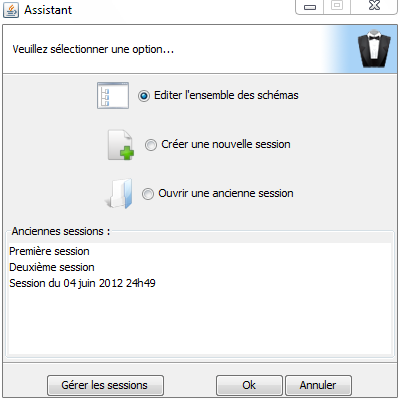
\includegraphics[width=0.6\textwidth]{../images/ouverture_session.png}
\caption{L'interface de gestion des sessions\\est accesible depuis l'assistant d'ouverture}
\end{figure}

\begin{figure}[h!]
\centering
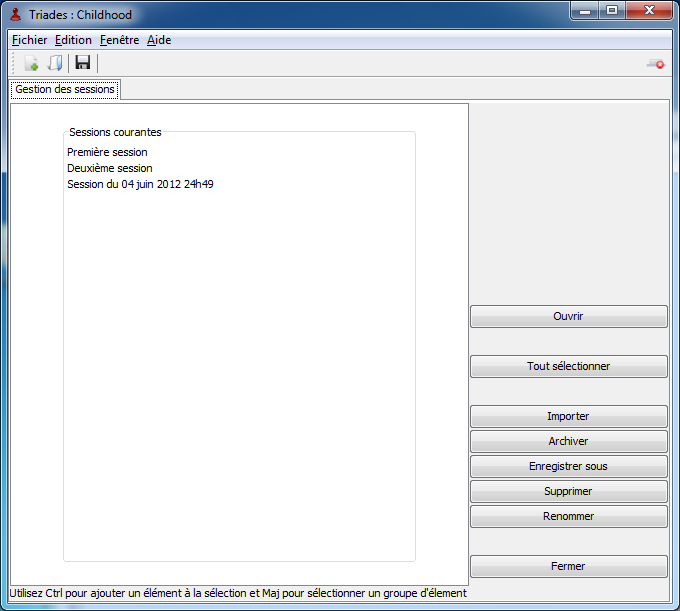
\includegraphics[width=0.8\textwidth]{../images/gestion_session.png}
\caption{L'interface de gestion des session}
\end{figure}

\subsection{Etiquettes par défaut des arêtes}
Il est possible de changer le contenu par défaut des étiquettes des arêtes dans les briques. Le sous-menu "Etiquettes des arêtes des briques" dans le menu Edition offre les possibilités suivantes :\\
\begin{itemize}
\item \textbf{Relations structurelles} : Affiche les 4 premiers caractères des relations structurelles de chaque temps d'action.\\
\item \textbf{Relations réelles} : De même avec les relations réelles.\\
\item \textbf{Relation au temps d'action : *} : Affiche la relation structurelle et la relations réelle pour le temps d'action sélectionné.\\ 
\end{itemize}

Cette option ne concerne que les relations dans les briques. Dans les exports, ces étiquettes sont contrôlées par les options globales de l'export (voir paragraphe \ref{globalExport}).\\

\begin{figure}[h!]
\centering
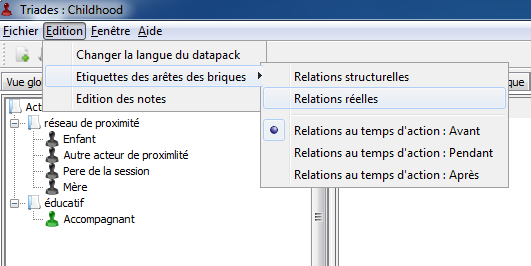
\includegraphics[width=0.5\textwidth]{../images/menu_edition.png}
\caption{Le menu de choix du contenu par défaut\\des étiquettes des arêtes}
\label{menu_edition}
\end{figure}

\subsection{Options globales lors d'un export}
\label{globalExport}
Le cadre présent sous l'arbre des acteurs sur la gauche de la fenêtre permet de contrôler plusieurs éléments portant sur l'ensemble de l'export.\\

Le premier champ permet de modifier le titre de l'export. Laisser ce champ vide masque le cadre de titre.\\

Le champ suivant permet de modifier les étiquettes par défaut des arêtes. Il est possible de masquer l'ensemble des arêtes avec l'option "Aucune étiquette". Cela permet de n'afficher que les étiquettes des arêtes modifiées manuellement.\\

Les deux champs suivants permettent de modifier la taille par défaut des étiquettes des sommets et des arêtes.\\

\begin{figure}[h!]
\centering
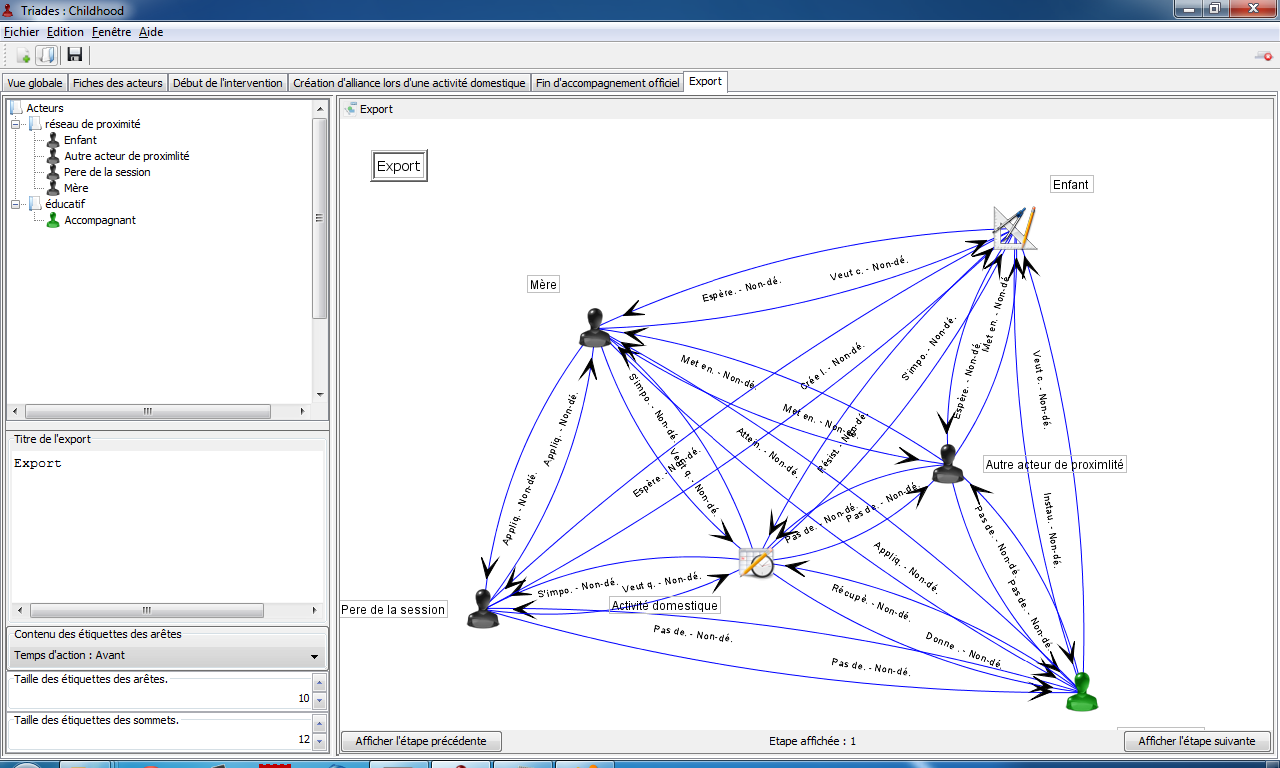
\includegraphics[width=0.5\textwidth]{../images/export_global.png}
\caption{Ces options se règlent à l'aide du cadre en bas à gauche de la fenêtre}
\end{figure}


\subsection{Edition des notes dans les briques}
Chaque brique est associée à une note. Cela permet d'ajouter des informations pour décrire une situation. Par défaut, les notes ne sont pas éditables. Il faut activer l'option "Edition des notes" dans le menu édition avant de pouvoir les modifier (voir image \ref{menu_edition}).\\

Les notes sont accessibles à l'aide du cadre présent en haut à droite de la zone d'affichage d'une brique. Attention, une note n'est accessible que dans la brique de la session où elle a été éditée. Elle ne sera pas accessible dans les autres sessions.\\

\begin{figure}[h!]
\centering
\begin{subfigure}{\textwidth}

\centering
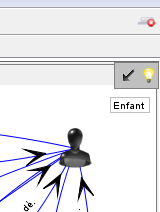
\includegraphics[width=0.4\textwidth]{../images/note_fermee.png}
\caption{Une note lorsqu'elle n'est pas affichée}
\end{subfigure}
\begin{subfigure}{\textwidth}

\centering
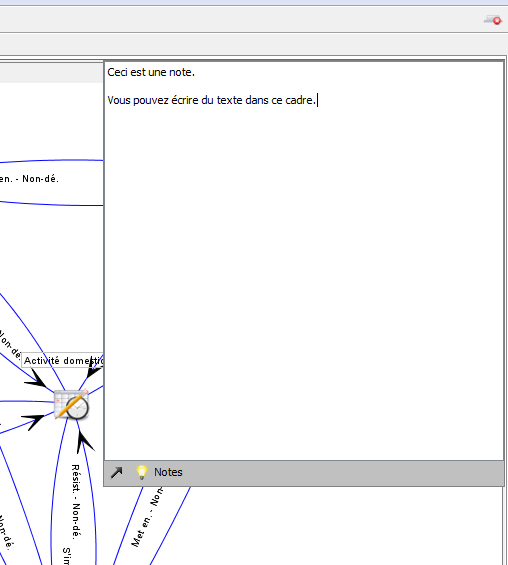
\includegraphics[width=0.4\textwidth]{../images/note_ouverte_edition.png}
\caption{Une note ouverte en cours d'édition}
\end{subfigure}
\begin{subfigure}{\textwidth}

\centering
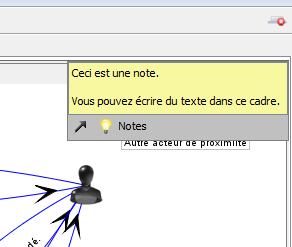
\includegraphics[width=0.4\textwidth]{../images/note_ouverte_pas_edition.png}
\caption{Une note en mode affichage uniquement}
\end{subfigure}
\caption{Différents états d'une note}
\end{figure}



\subsection{Gestion des traductions de datapack}
Il possible d'importer et d'exporter une traduction depuis le module de traduction.\\

Attention, lors d'une importation, la traduction est perdue. Veillez à exporter cette dernière avant si vous voulez la conserver.\\

Il est aussi possible de changer la traduction depuis le datapack avec l'option "Changer la langue du datapack" dans le menu Edition (voir image \ref{menu_edition}). De même, la traduction actuelle sera écrasée lors de cette opération.\\



\section{Version 1.0.2}
\subsection{Suppression d'un export}
Il est maintenant possible de supprimer un export en faisant un clic droit sur l'export à supprimer dans l'arbre de la vue globale. Attention, l'export peut rester dans la liste jusqu'au prochain lancement du logiciel.\\ 


\subsection{Statistiques des traductions}
De plus, un bouton "Statistiques de la traduction" permet d'obtenir le compte des mots d'une traduction. Cela permet de chiffrer facilement le coût de la traduction.\\ 

\section{Version 1.0.3}
\subsection{Choix de la langue de l'interface}
La langue de l'interface peut être choisie à l'aide du menu "Langue" dans l'interface principale. Le logiciel doit être redémarré après un changement de langue.\\

Il est possible d'ajouter une nouvelle langue en ajoutant le fichier correspondant dans le sous dossier "language" du répertoire d'installation du logiciel. Pour réaliser cette traduction, il suffit de réaliser une copie d'un des fichier puis de traduire l'ensemble des phrases qu'il contient. La nouvelle langue sera proposée dans le menu "Langue" lors du démarrage suivant du logiciel.\\

Si des phrases sont manquantes dans un fichier de traduction, celles de la version françaises seront automatiquement utilisées à la place. De ce fait, si certaines phrases sont en français, cela signifie sûrement que leur traduction est manquante. 

\subsection{Téléchargement et mise à jour automatique du datapack}
Lors du premier lancement de la version étudiante, l'utilisateur est invité à saisir une adresse à laquelle le datapack peut être téléchargé. En effet, le logiciel en version étudiante est initialement fourni sans datapack afin de permettre un déploiement plus aisé de nouvelles sessions ou d'une traduction locale du contenu du datapack. Il est possible qu'il soit nécessaire de relancer le logiciel une fois le fichier téléchargé.\\

\subsubsection{Programme AutoUpdater}
Le programme "AutoUpdater" permet de mettre à jour automatiquement le datapack à partir d'un fichier téléchargé sur internet.\\

Lors du lancement de l'AutoUpdater, l'utilisateur est invité à saisir l'adresse de téléchargement du datapack. Dans le cas où le datapack courant et le nouveau contiennent une traduction ou des sessions portant le même nom, le programme demande à l'utilisateur quelle version il souhaite conserver.\\

Une sauvegarde de l'ancien datapack est automatiquement réalisée et placée dans le dossier "datapack\_backup".



\subsection{Saisie d'une licence d'utilisation}
Les datapacks fournis avec la version étudiante du logiciel ont un durée d'utilisation limitée dans le temps. Lors de l'achat d'une licence, un code de déblocage du datapack est fourni. Ce code peut être saisi à l'aide de l'option "Enregistrer une licence". Une fenêtre s'ouvre alors invitant l'utilisateur à saisir l'adresse mail associée à la licence puis le code de validation.\\

Lors de l’utilisation d'un datapack dont la durée d'essai s'est achevé, une boite de dialogue invite l'utilisateur à saisir ces mêmes informations pour permettre l'utilisation du datapack. Il est possible qu'un redémarrage du logiciel soit nécessaire lors de la saisie d'une licence.\\

\subsection{Fonctions dédiées à la version enseignant}
\subsubsection{Génération de licences et de datapacks limités dans le temps}
Le menu "Outils", uniquement présent dans la version enseignant du logiciel, permet de générer des licences d'utilisation ainsi que d'exporter des datapack à destination des versions étudiantes.

Lors de l'utilisation de ces deux outils, il vous est demandé de saisir votre clé personnelle. Cette dernière vous a normalement été fournie lors de la livraison du logiciel.\\

\paragraph{Génération de licences}
La génération de licences se déroule en deux étapes. Tout d'abord, l'utilisateur doit saisir la liste des adresses mails pour lesquelles une licence doit être générée. Il est possible d'extraire cette liste depuis le presse-papier. Dans ce cas, les séparateurs utilisés sont au choix : la virgule, le point-virgule, la tabulation et le retour chariot. Cela permet en particulier d'importer facilement cette liste depuis un tableur.\\
Il est aussi possible d'ajouter une adresse à l'aide du champ mail et du bouton juste à sa droite situé en haut de la fenêtre. Les différentes entrées pouvant être modifiées et supprimées à l'aide des boutons dédiés en haut à droite de la fenêtre.\\
Le type de licence peut être choisi à l'aide de la liste à puce en bas de la fenêtre. Il n'est pas possible de spécifier plusieurs licences différentes pour une même liste. L'option "Licence déjà facturée" permet de générer à nouveau un code de licence au cas ou ce dernier aurait été perdu par l'utilisateur.\\

L'étape suivante consiste à générer les licences. Attention, un connexion internet sera nécessaire lors de cette étape. Le processus est lancé lors du clic sur le bouton "Générer les licences". La liste de mail ne sera plus modifiable par la suite.\\

L'utilisateur est invité à choisir le lieu d'enregistrement du fichier de licence dans lequel il veut stocker le récapitulatif des licences générés. Il est ensuite possible de copier au choix une adresse mail, un code de déblocage, un couple mail/code de déblocage ou la liste entière à l'aide des boutons situés sur la droite de la fenêtre.\\

Une fois la fenêtre de génération des licences fermées, il n'est plus possible d'accéder à la liste générées au sein du logiciel, mais uniquement grâce au fichier récapitulatif créé lors de la génération.\\

Une demande de facturation est automatiquement envoyé à l'équipe de développement lors de la génération des licences.

\paragraph{Génération d'un datapack pour les version étudiantes}

L'autre option du menu outils permet de générer des datapack pour les versions étudiantes du logiciel. Lors de cette opération, l'utilisateur est tout d'abord invité à saisir la durée de validité du datapack. La durée maximale est de 365 jours. La durée minimale est 0 jours, cela correspond à un datapack bloqué immédiatement. Ce type de datapack est destiné à être mis à disposition des utilisateurs ayant acheté une licence d'utilisation afin qu'(il puisse le télécharger lors d'une réinstallation ultérieure du logiciel.\\

La fenêtre suivante invite l'utilisateur à choisir l'endroit ou le datapack devra être enregistré.\\

Une fois l'emplacement choisi, le datapack est automatiquement exporté.\\


\end{document}

